\documentclass[11.5pt]{article}
\usepackage[utf8]{inputenc}
\usepackage{amsmath,amssymb,amsthm,enumerate,float,geometry,latexsym,bm}
\usepackage{kpfonts}
\usepackage{hyperref}
\usepackage{apacite}
\usepackage{epigraph}
\usepackage{booktabs}
\usepackage{graphicx}
\usepackage{tikz}
\usepackage{caption}
\usepackage{multirow}

\usetikzlibrary{shapes.geometric,positioning}
\usepackage{pgfplots}
\usepackage[misc]{ifsym}

% Enhanced document geometry
\geometry{letterpaper, margin=1in}

% Spacing and paragraph formatting
\setlength{\parindent}{0.5in}
\setlength{\parskip}{6pt}
\linespread{1.5}

% Title and author information
\title{SNAP PROJECT}
\author{Alejandro Herrera-Caicedo \& Inder Majumdar}
\date{June 2025}

\begin{document}

% Title page
\maketitle
\begin{abstract}
  
    
\end{abstract}










% Data ---------------------------------------------------------------------------------------------------------------------------------------

\section{Other Policies With Gaming}

\begin{itemize}
  \item \textbf{SNAP ABAWD waivers.} States may combine contiguous counties/economic regions and document a group unemployment rate (e.g., recent 12-month $>10\%$ or 24-month average $\ge 120\%$ of the national rate) to waive work-time limits. States have discretion in defining the combined area subject to FNS review. 

  \item \textbf{School meals – Community Eligibility Provision (CEP).} Districts can qualify a \emph{group of schools} if the group’s Identified Student Percentage (ISP) is at least 25\% (final rule, Sept.\ 26, 2023); individual schools within the group may be below 25\%.

  \item \textbf{Opportunity Zones.} Governors could nominate up to 25\% of eligible low‑income tracts, plus up to 5\% of nominations for contiguous non‑low‑income tracts meeting income limits—allowing tract sets that include some otherwise ineligible tracts. 

  \item \textbf{SBA HUBZone – Governor‑Designated Covered Areas (GDCAs).} In addition to standard census‑based designations, governors may petition SBA to designate rural/high‑unemployment areas as HUBZones. 

  \item \textbf{Health workforce shortages – MUA/HPSA.} Applicants define a \emph{Rational Service Area} (often grouped tracts/counties). MUAs qualify with IMU $\le 62$; service‑area delineation affects eligibility. 

  \item \textbf{HUD CDBG “Urban Counties.”} Counties can aggregate unincorporated areas plus participating units to meet the \textasciitilde200{,}000 population test for entitlement status.

  \item \textbf{EPA NAAQS nonattainment boundaries.} States propose multi‑county boundaries; EPA designates areas using factors (monitors, emissions/transport, meteorology, geography, jurisdictional lines). 

  \item \textbf{EDA distress eligibility.} Projects may qualify at county, multi‑county, or neighborhood scales using unemployment or income thresholds; public tools support testing regional combinations. 

  \item \textbf{WIOA local workforce areas / ASU.} States designate local areas with local officials; funding formulas and “Areas of Substantial Unemployment” depend on area definitions and statistics. 

  \item \textbf{Medicare hospital wage index reclassification (MGCRB).} Hospitals (and some statewide group efforts) can reclassify to another wage area if distance and wage‑similarity tests are met, changing payment thresholds. 
\end{itemize}



\section{Virginia}
Surprisingly we observe that the lagged unemployment rate yields a negative discontinuity on the probability of treatment, while other observables remain more or less the same. 

\begin{figure}[h!]
    \centering
    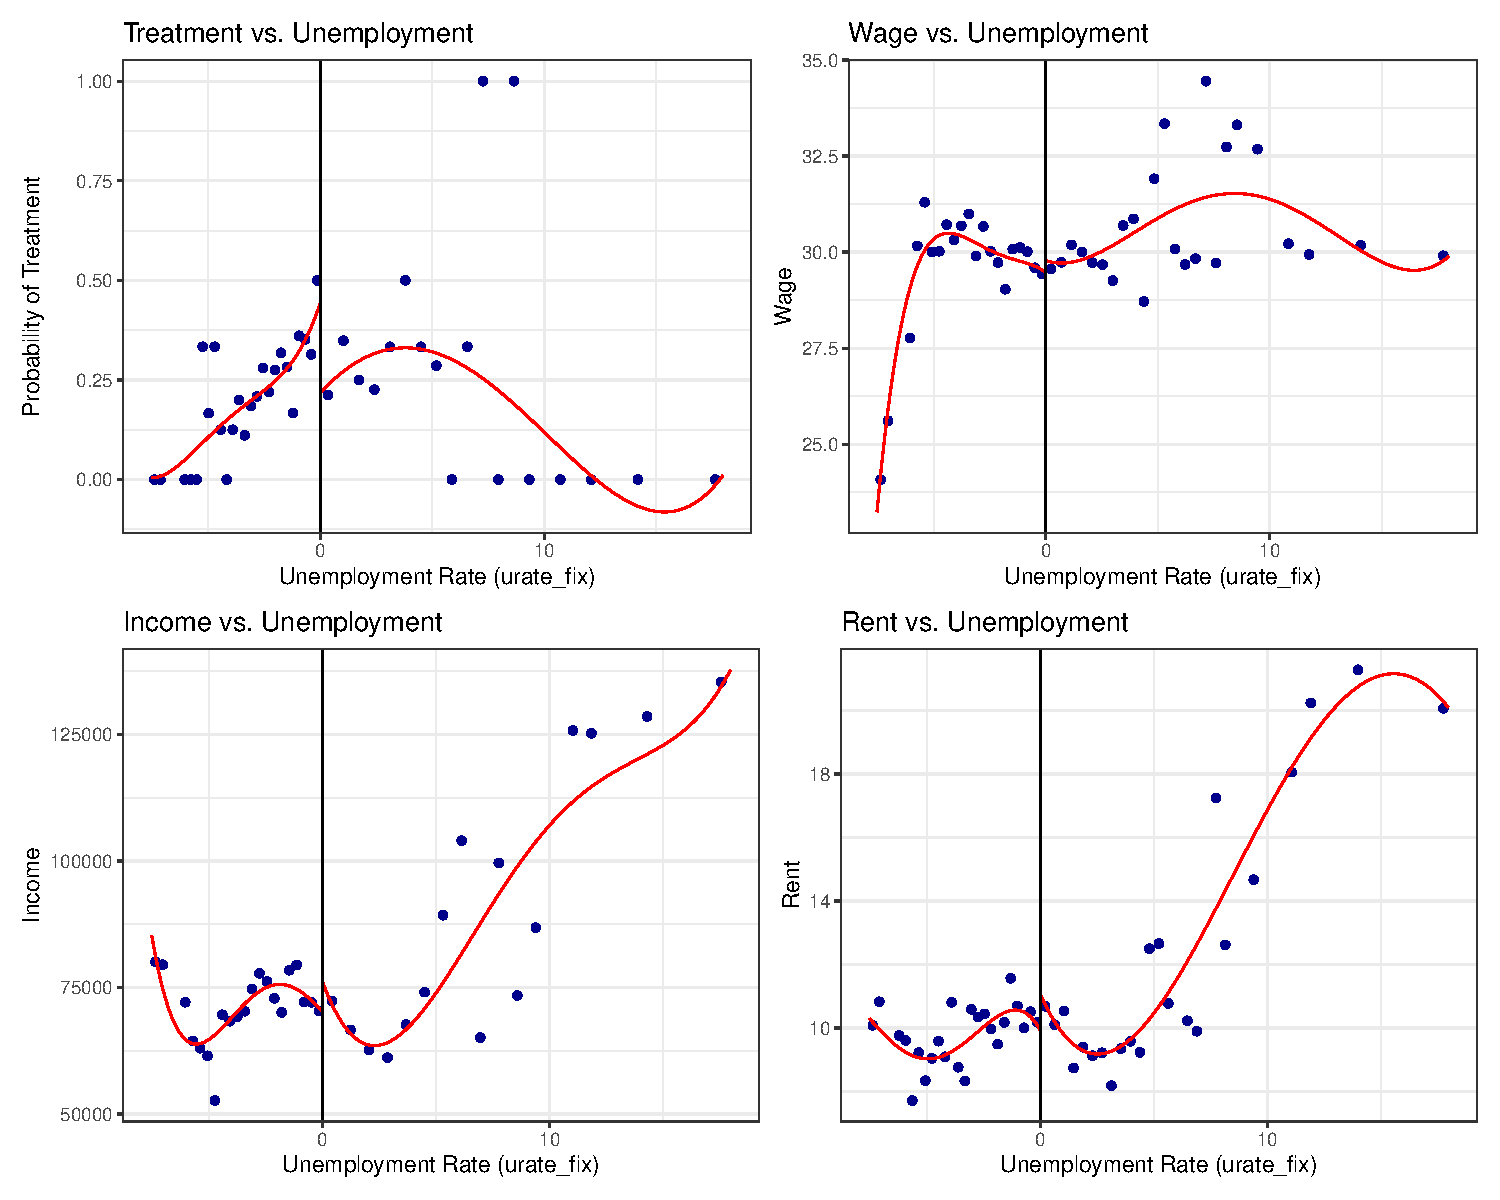
\includegraphics[width=0.75\linewidth]{Figures/cutoffs_virginia.pdf}
    \caption{Virginia's Cutoffs}
    \label{fig:enter-label}
\end{figure}
% From the TWFE/SA(21) estimates we observe that from 2014-2019 window there is an increase in dollar stores in the presence of the ABAWD waivers. Waivers are assigned at a region level, where a region needs to have an unemployment higher than 10\%. This should mean that in principle we should observe individual counties above 10\% to be always treated, but the ones below the threshold are not necessarily going to serve as a control, as they can be binned in an area. This could explain why the discontinuity yield an increase of 19\% in the likelihood of being treated, but it is not significant. Similarly, local effect of dollar store entry is weaker and very noisy.

% \begin{table}[H]
% \centering
% \begin{tabular}{llccccc}
% \toprule
% \textbf{Outcome} & \textbf{Method} & \textbf{Coef.} & \textbf{Std. Err.} & \textbf{$z$} & \textbf{P-value} & \textbf{95\% CI} \\
% \midrule
% Waiver             & Conventional & 0.191 & 0.198 & 0.968 & 0.333 & [-0.196, 0.578] \\
% Waiver             & Robust       & --    & --    & 1.246 & 0.213 & [-0.157, 0.704] \\
% $\text{ihs}(\#\text{DS})\approx\log(\#\text{DS})$ & Conventional & 0.062 & 0.141 & 0.442 & 0.659 & [-0.214, 0.338] \\
% $\log(\#\text{DS})$  & Robust       & --    & --    & 0.575 & 0.565 & [-0.230, 0.422] \\
% \bottomrule
% \end{tabular}
% \caption{Sharp RD estimates for Waiver Status and Dollar Store Entry}
% \label{tab:rd_stacked}
% \end{table}



% A IV implementation (using unemployment) yields a similar issue. Where the coefficient is positive but insignificant. 

% \begingroup
% \centering
% \begin{tabular}{lcccc}
%    \toprule\toprule
  
%    Dependent Variable:  & \multicolumn{2}{c}{{Full Sample}} & \multicolumn{2}{c}{{Near Discontinuity}} \\
%    Model:        & (1)      & (2)      & (3)      & (4)\\  
%    \midrule
%    \emph{Variables}\\
%    treatment     & 0.3688   & 0.7193   & 1.687    & 1.241\\   
%                  & (0.3309) & (0.7416) & (3.088)  & (3.737)\\   
%    wage          & 0.0061   & 0.0082   & -0.0074  & -0.0124\\   
%                  & (0.0121) & (0.0142) & (0.0638) & (0.0582)\\   
%    \midrule
%    \emph{Fixed-effects}\\
%    county\_fips  & Yes      & Yes      & Yes      & Yes\\  
%    year          & Yes      & Yes      & Yes      & Yes\\  
%    \midrule
%    \emph{Fit statistics}\\
%    Observations  & 798      & 798      & 150      & 150\\  
%    R$^2$         & 0.28636  & 0.18392  & -0.16194 & 0.12641\\  
%    Within R$^2$  & -0.03128 & -0.17931 & -0.88264 & -0.41544\\  
%    \bottomrule\bottomrule
%    \multicolumn{5}{l}{\emph{Clustered (county\_fips) standard-errors in parentheses}}\\
%    \multicolumn{5}{l}{\emph{Signif. Codes: ***: 0.01, **: 0.05, *: 0.1}}\\
% \end{tabular}
% \par\endgroup

% The argument for this is that the discontinuity is not at the individual level, but at "being the last picked" to become part of an area. 

% References
\newpage
\bibliography{references}
\bibliographystyle{apacite}



\end{document}
